\addcontentsline{toc}{section}{Introduction}
\section*{Introduction}

Dans ce chapitre, nous explorerons la schématisation détaillée du projet visant à remplacer notre architecture monolithique par une approche basée sur des microservices et des micro-frontends, tout en migrer notre système de gestion de base de données de MariaDB vers Delta Lake. Cette transition marque une étape cruciale dans notre parcours d'évolution technologique, offrant des avantages significatifs en termes de flexibilité, d'évolutivité et de maintenabilité.

\section{Smart Data}

La smart data fait référence au processus d'extraction d'informations précieuses à partir de grandes quantités de données afin de prendre des décisions commerciales éclairées.

La smart data nous permet de:

\begin{enumerate}
    \item \textbf{Collecte des données}: Izicap aide les entreprises à collecter des données clients à partir de différents points de contact tels que les systèmes de point de vente, les programmes de fidélité, les interactions en ligne, etc. Assurez-vous d'intégrer leurs outils de collecte de données dans vos systèmes ou processus existants.
    \item \textbf{Analyse des données}: La solution de smart data d'Izicap vous permet d'analyser les données collectées pour découvrir des tendances, des modèles et des comportements clients. Utilisez leurs outils d'analyse et leurs algorithmes pour obtenir des informations exploitables à partir des données.
    \item \textbf{Segmentation des clients}: Segmentez votre base de clients en fonction de leurs préférences, de leur historique d'achat, de leurs caractéristiques démographiques ou d'autres critères pertinents. La solution de smart data d'Izicap peut vous aider à identifier différents segments de clients et à créer des stratégies marketing personnalisées pour chaque segment.
    \item \textbf{Marketing personnalisé}: Exploitez les informations tirées de la solution de smart data d'Izicap pour créer des campagnes marketing ciblées. Envoyez des offres personnalisées, des promotions ou des recommandations à des segments spécifiques de clients, augmentant ainsi les chances de conversion et de satisfaction client.
    \item \textbf{Fidélisation de la clientèle}: Utilisez la solution de smart data d'Izicap pour identifier les clients qui risquent de résilier leur abonnement ou de ne plus acheter chez vous. Développez des stratégies de fidélisation en leur offrant des incitations, des programmes de fidélité ou des communications personnalisées afin de les maintenir engagés et fidèles à votre marque.
    \item \textbf{Suivi des performances}: Surveillez régulièrement les performances de vos campagnes marketing et de vos efforts d'engagement client. La solution d'Izicap peut vous fournir des métriques et des rapports pour évaluer l'efficacité de vos stratégies et apporter des ajustements basés sur les données lorsque nécessaire.
    \item \textbf{Amélioration continue}: Les solutions de smart data sont les plus efficaces lorsqu'elles sont utilisées de manière itérative. Analysez régulièrement les données, adaptez vos stratégies et peaufinez votre approche en fonction de nouvelles informations et de l'évolution du comportement client.
\end{enumerate}


\begin{figure}[H]
\centering

\includegraphics[width=0.6\linewidth]{images/smart-data-izicap.png}
\caption{Smart data Izicap}\label{fig:smart-data-Izicap}
\end{figure}


\section{L'architecture du système}

La figure ci-dessous visualise la structure et les composants clés de notre système, ainsi que les interactions entre eux, elle constitue ainsi le fondement de notre système et joue un rôle essentiel dans la fourniture de fonctionnalités et de services à nos utilisateurs.

\begin{figure}[H]
\centering
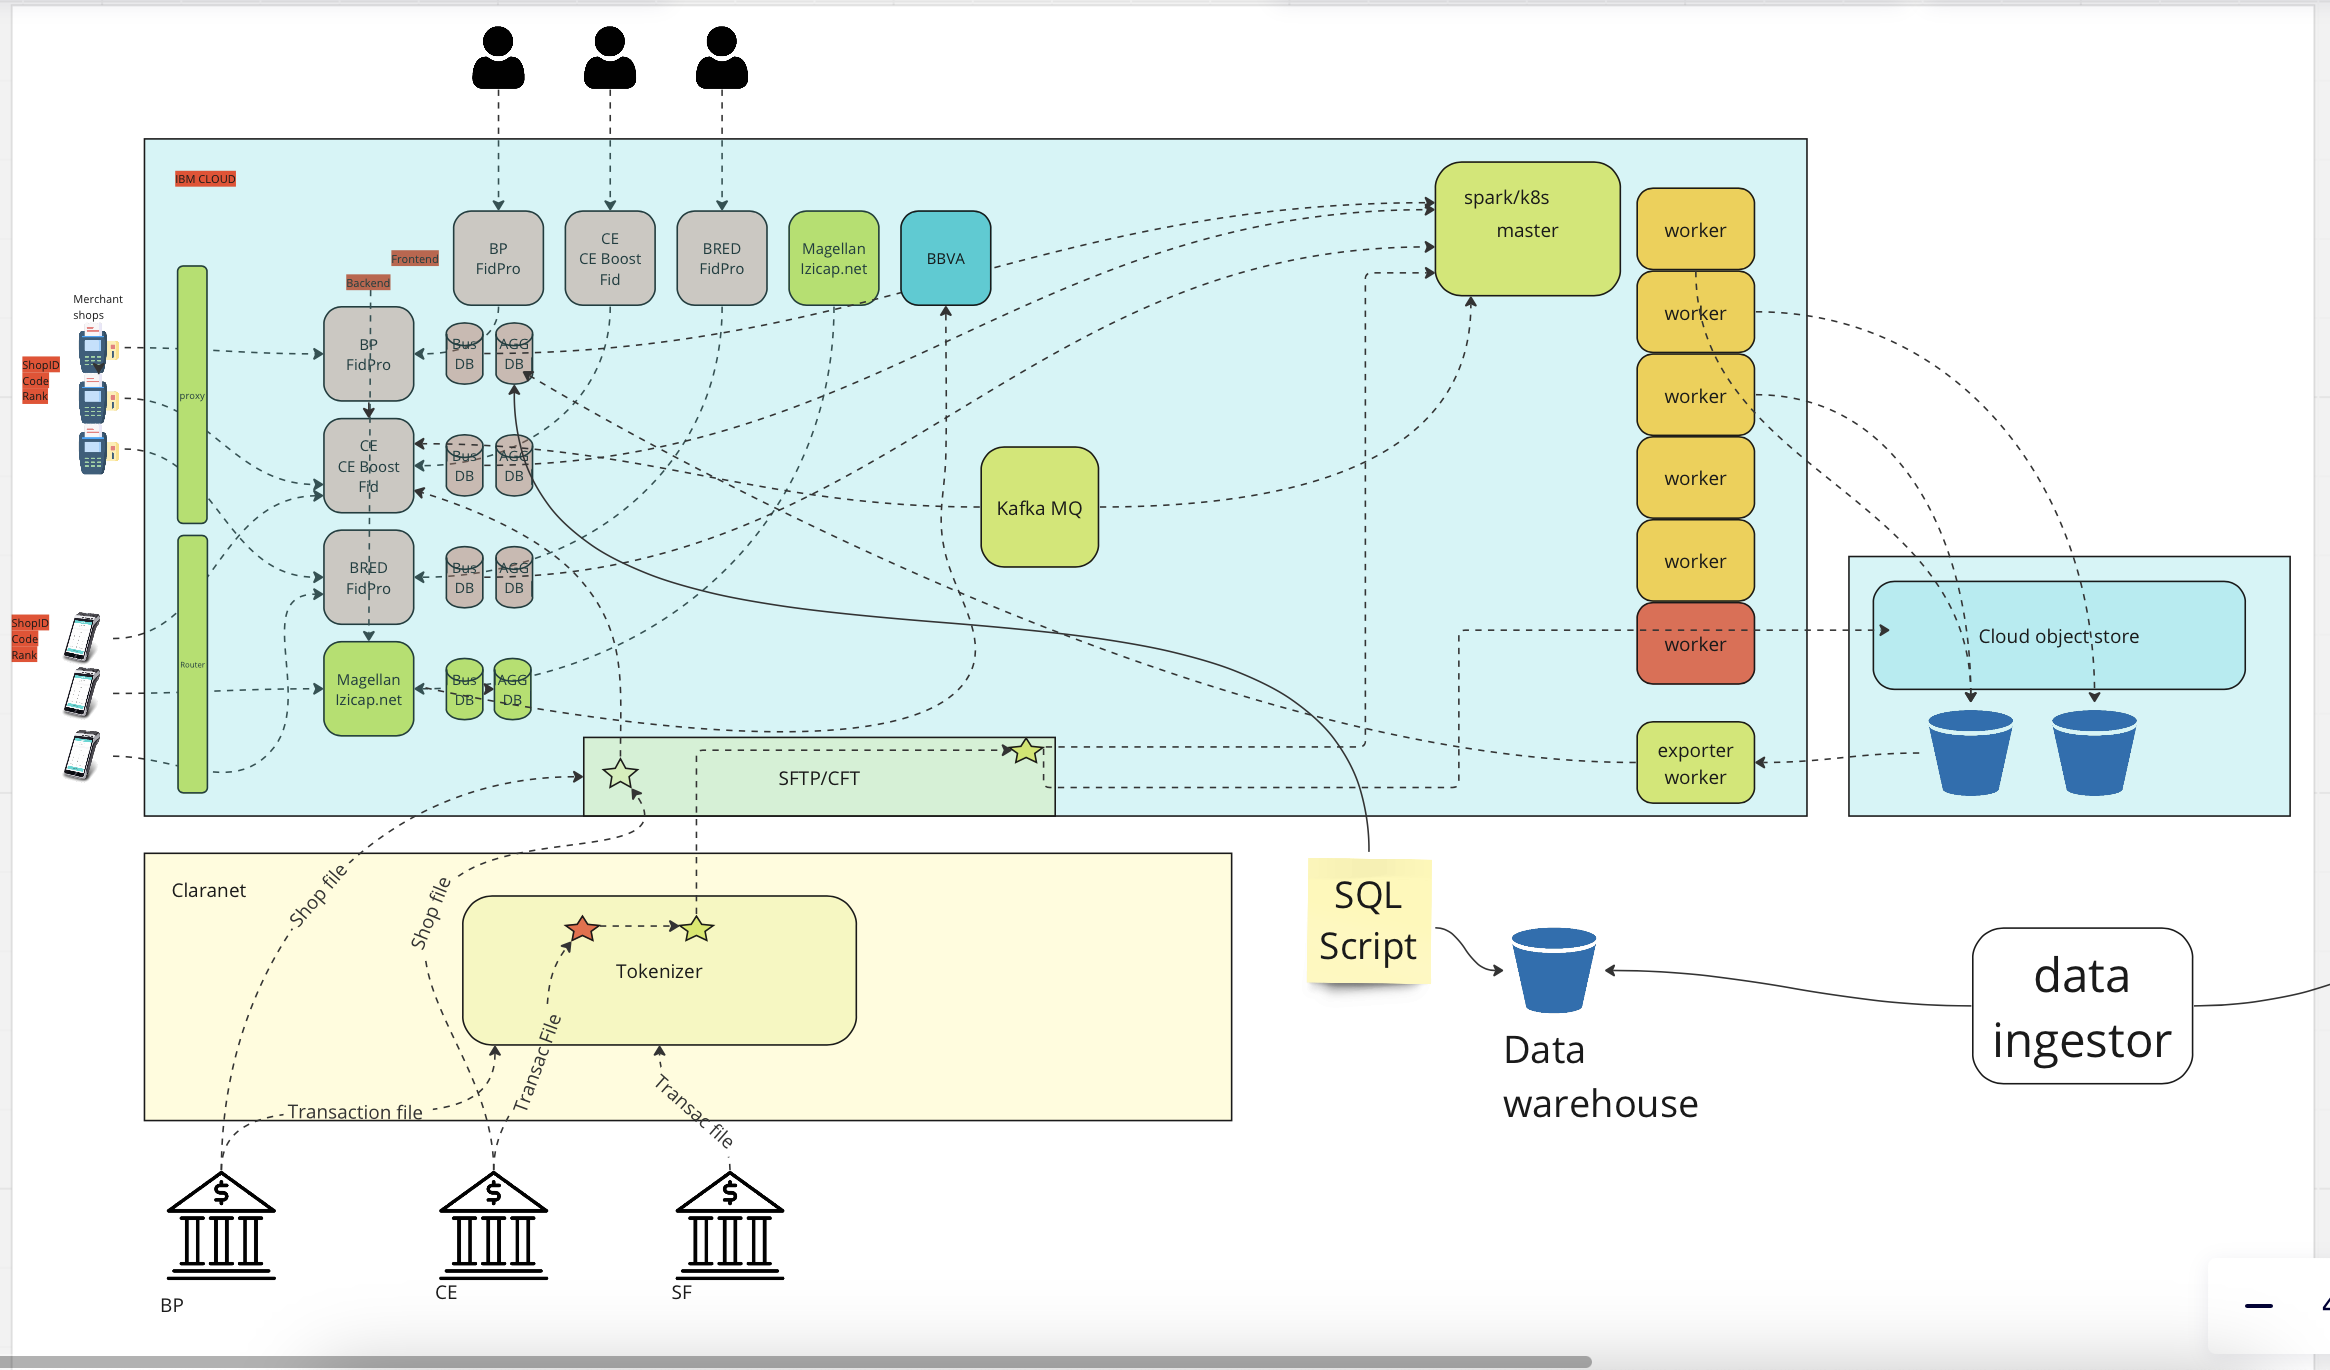
\includegraphics[width=\linewidth]{images/archi-globale.png}
\caption{Architecture du système actuelle}\label{fig:architecture-monolithique}
\end{figure}

Ce schéma représente le fonctionnement de l'architecture monolithique actuelle qui présente plusieurs inconvénients qui peuvent entraver l'efficacité, la flexibilité et la maintenabilité du système. Voici une description détaillée des principaux inconvénients:

\begin{enumerate}
    \item \textbf{Complexité et dépendances}: L'architecture monolithique implique que tous les modules et fonctionnalités du système sont regroupés en un seul bloc. Cela crée une forte interdépendance entre les différents composants, rendant la compréhension, la gestion et les mises à jour complexes. Les modifications apportées à une partie du système peuvent avoir des répercussions sur d'autres parties, ce qui rend les tests, les déploiements et les corrections d'erreurs plus difficiles.
    \item \textbf{Scalabilité limitée}: L'architecture monolithique a souvent des difficultés à s'adapter à une augmentation de la charge ou à une demande croissante. Étant donné que tous les composants sont regroupés dans un seul monolithe, il est difficile de faire évoluer sélectivement une partie spécifique du système. Cela peut entraîner des goulots d'étranglement, des performances réduites et une mauvaise répartition des ressources lorsqu'il s'agit de traiter des volumes de données importants ou de gérer une augmentation du nombre d'utilisateurs.
    \item \textbf{Déploiements complexes et risques élevés}: Avec une architecture monolithique, les déploiements nécessitent la mise à jour de l'ensemble du système, même pour des modifications mineures. Cela augmente les risques d'erreurs et de régressions, car une seule erreur peut entraîner l'indisponibilité du système tout entier. De plus, les déploiements doivent être soigneusement planifiés et coordonnés, ce qui peut entraîner des temps d'arrêt plus longs et des interruptions de service pour les utilisateurs.
    \item \textbf{Difficulté de choix technologiques}: Dans une architecture monolithique, les technologies utilisées sont souvent liées et intégrées de manière étroite. Cela peut rendre difficile l'adoption de nouvelles technologies ou l'intégration de composants spécialisés. Les mises à niveau de versions ou les ajouts de nouvelles fonctionnalités peuvent être limités par les choix technologiques initiaux, ce qui peut entraver l'innovation et l'adaptation aux évolutions du marché.
    \item \textbf{Cohésion et responsabilités}: L'architecture monolithique ne facilite pas une séparation claire des responsabilités et des fonctionnalités. Les différents modules du système sont souvent intimement liés et peuvent partager des fonctionnalités communes. Cela rend difficile l'isolation des problèmes, la maintenance spécifique des modules et la réutilisation de code spécifique à un domaine.
\end{enumerate}


\section*{Conclusion}
\addcontentsline{toc}{section}{Conclusion}

Delta Lake est un outil important pour le traitement du Big Data, fournissant une gestion fiable des données et garantissant l'intégrité des données à grande échelle. Ses transactions ACID, l'application des schémas et les fonctionnalités de gestion des versions des données en font un choix populaire pour les entreprises qui doivent traiter de grandes quantités de données avec une grande précision et fiabilité.

En utilisant Delta Lake, les ingénieurs de données et les scientifiques des données peuvent facilement gérer la qualité des données, suivre la lignée des données et collaborer sur des projets d'analyse de données. Grâce à son intégration transparente avec d'autres outils de Big Data. Delta Lake fournit une solution puissante pour le traitement du Big Data qui peut aider les entreprises à mieux comprendre leurs données plus rapidement et plus efficacement.